\documentclass[10pt,journal,compsoc]{IEEEtran}
\usepackage{blindtext}
\usepackage{multicol}
\usepackage{listings}
\usepackage{graphicx}
\usepackage{wrapfig}
\usepackage{float}
\graphicspath{ {./images/} }
\usepackage[english]{babel}

\usepackage{graphicx} % package for including graphics
\usepackage{amsmath} % package for using mathematical symbols
\usepackage{amssymb} % package for using additional mathematical symbols
\usepackage{subfig} % package for including multiple figures on one page
\usepackage{url}
\usepackage{booktabs}
\usepackage{tabularx}
\usepackage[hidelinks]{hyperref}
\usepackage{color}

\usepackage{xcolor}
\usepackage{float}
\usepackage{graphicx}
\usepackage[utf8]{inputenc}
\usepackage{shortcut}
\usepackage{enumitem}

\usepackage{array}
\usepackage{multirow}
\usepackage{multicol}
\usepackage{boldline}
\usepackage{hhline}

\begin{document}

\definecolor{azulUC3M}{RGB}{0,0,102}

\begin{titlepage}
    \begin{sffamily}
        \color{azulUC3M}
        \begin{center}
            \begin{figure}[H] %incluimos el logotipo de la Universidad
                \makebox[\textwidth][c]{
\includegraphics[width=16cm]{Portada_Logo.png}}
            \end{figure}
            \vspace{2.5cm}
            \begin{Large}
                Master in Cybersecurity\\
                2022-2023\\
                \vspace{2cm}
                \textsl{Master's Thesis}
                \bigskip

            \end{Large}
            {\Huge \textbf{``Secure speedup of the future JavaScript deployments''}\\
            \vspace*{0.5cm}
            \rule{10.5cm}{0.1mm}\\
            \vspace*{0.9cm}
            }
            {\LARGE {Aitor Ruiz Garcia}\\
            \vspace*{1cm}
            }
            \begin{Large}
                Director\\
                Pedro Peris López\\
                Madrid, 2023\\
            \end{Large}
        \end{center}
        \vfill
        \color{black}
        
\includegraphics[width=4.2cm]{creativecommons.png}\\
        Esta obra se encuentra sujeta a la licencia Creative Commons \textbf{Reconocimiento - No Comercial - Sin Obra Derivada}\\
    \end{sffamily}
\end{titlepage}

\title{Secure speedup of the future JavaScript deployments}
\author{\IEEEauthorblockN{Aitor Ruiz Garcia*}\\
    \IEEEauthorblockA{\textit{Master in Cybersecurity, Universidad Carlos III de Madrid}}
    \thanks{*Corresponding author.}% <-this % stops a space
    \thanks{\textit{E-mail address:}100482217@alumnos.uc3m.es}}

\date{September 2023}
\maketitle
\section{Abstract}
JavaScript has emerged as a fundamental language in global development. Much of the success of Node.js, both in server-side applications and in full-stack web applications (client-server), can be attributed to it.

Node.js was primarily created to enable JavaScript to run on the server. The creator of Node never anticipated that JavaScript would be used for literally everything.

JavaScript is employed in desktop applications using Electron \cite{ELECTRON}, and in mobile applications using React Native \cite{RN} or Ionic \cite{IONIC}. As an interpreted language, it has a low entry barrier. As the default language of the web, it also boasts a wealth of interesting libraries.

Node.js took the engine that runs JavaScript on Chrome, known as V8, and wrapped it in additional C++ code to make it possible for it to interact with system calls \cite{FKNODE}.

All these factors have contributed to the rise of JavaScript as the language of the future. Nonetheless, as the creator himself contends, it has experienced some 'growing pains' \cite{FKNODE}.

This project is born with the idea of solving some of these problems. The main objective is to create a library that can be used in Deno projects to speed up the most common operations. This library will be written in Rust, a language that is both fast and memory safe.

This operations will be cryptographic operations, such as hashing, encrypting and decrypting. These operations are very common in the web space, and they are very CPU intensive. This is why they are a good candidate for this project.

\section{The problem}

Ryan Dahl, the creator of Node.js, has expressed his regrets about the language \cite{FKNODE}. He has stated that he would not use JavaScript for a new project and that he would also not use Node.js for a new project. Node.js has grown beyond what it was intended to be, and it has become a 'monster'.

While experimenting with the TFG \cite{TFG} project, some problems where experienced with the current state of the JavaScript ecosystem, which they will be explained in the following sections. This TFG project was a web application with blockchain integrations for decentralized identity management. Even though this project is not within the scope of this TFM, it is important to understand the context of the problems that I have discovered.

\subsection{No types}
JavaScript does not have a type checker, at least at \textit{compile} time. JavaScript is an interpreted language, therefore it does not have a compile step. This means that there is no compiler to check the types of the variables, and therefore, it is possible to assign a value of one type to a variable of another type. This can lead to unexpected errors in the code. It is also possible to request a property from an object that does not exist. This will result in a runtime error, with no previous warning.

Take a look at the following example:
\begin{lstlisting}
const user = {
    name: "",
    age: 0
}
    
console.log(user.email);
\end{lstlisting}

This small code will not raise any error to warn the developer that the user object does not have an email property. This leads to a runtime error, which is not good for the developer experience.

It is even worse when the user receives the error in production, because the error will be shown to the user, and the user will not understand what is happening.

This happens because JavaScript is a dynamic language and does not have a type checker.

The original TFG \cite{TFG} employed Next.js, a popular framework for server-rendered React applications. Initially, the challenges that are elaborated in subsequent sections were not foreseen. Next.js was chosen due to familiarity with the framework. However, as the project evolved, issues began to arise, particularly related to the absence of types.

\subsection{node\_modules}

Node.js has a package manager called npm. This package manager is used to install libraries in the project. The problem is that the libraries are installed in the \verb|node_modules| folder, and this folder can grow significantly. \cite{BADNPM}

By default, npm does not create symbolic links between the libraries. This means that if you have two libraries that use the same dependency, that dependency will be installed twice. More packages installed means more disk space used and more time required to install the packages. A CI build could take a considerable amount of time just to install all the packages.

\subsubsection{node\_modules security implications}

As JavaScript is mainly used in web applications, both on the server and in the client, it is a good target for attacks. Currently, npm holds more than 1.6 million packages. \cite{NPMCOUNT}

A successful attack on a web framework could grant access to a large number of browsers, a small percentage of which may be vulnerable.

Although JavaScript in a browser is sandboxed, making it \textit{safer}, this is not the case with Node.js. In Node.js, all the code can interact with the file system and the entire internet.

In the past, there have been multiple cases of compromised npm packages, the most famous being \verb|colors| and \verb|faker.js|. \cite{BADFAKER} \cite{VERGEFAKER}

The developer went rogue and introduced infinite loops, disrupting the normal workflow of multiple developers.

Another notable example was \verb|UAParser.js|, which downloaded and installed a password stealer and a cryptominer. It is important to note that this package is still used by millions of users daily.


\subsection{Node GYP}

Node GYP is the state of the art when creating native libraries in Node JS. This tool is originally from google \cite{FKNODE}. When google discontinuated it the comunity made a fork and the project continued. \cite{NODEGYP}

It is a tool writen in python, witch is not JavaScript, and it is inecessarilly complicated to write a native library.

In order to create a native library, some deep \verb|C++| understanding is needed and the tooling around it is writen in a variety of languagues making it an extra effort to develop some native libraries.

In the original repository they present a simple example of a native library. \cite{NODEGYP}

It consists of 33 lines of code for a simple Hello world.

\begin{lstlisting}
extern "C" NODE_MODULE_EXPORT void
NODE_MODULE_INITIALIZER(
    v8::Local<v8::Object> exports,
    v8::Local<v8::Value> module,
    v8::Local<v8::Context> context) {
  NODE_SET_METHOD(exports, "hello", Method);
}
\end{lstlisting}

It needs a lot of boiler plate code just to signal the actual function it is going to be called from JavaScript.

\begin{lstlisting}
static void Method(
    const v8::
    FunctionCallbackInfo<v8::
    Value>& 
    args
    ) {
  v8::Isolate* isolate = args.GetIsolate();
  args.GetReturnValue()
    .Set(
        v8::String::NewFromUtf8(
        isolate, 
        "world")
        .ToLocalChecked()
    );
}
\end{lstlisting}

It requires to interact with the V8 engine directly, witch is not a trivial task. This code, even though it is simple, it is not easy to understand. It just returns a string with the value \verb|world|.

This code will be more complicated in some other C ABI compatible languages, because they would need to implement the V8 engine in their language, to then be able to interact with it.

Rust, that will be discused later has a crate that links directly with V8, but it is not a trivial task to implement.

\section{The solution}

Ryan Dahl, created Deno, a solution to his own issues created by working on Node JS without a clear plan. In a talk at JSConf \cite{FKNODE} he presented the project with some clear plan to make Deno the standard langua for the web.

His plan was to create a safe and secure environment for JavaScript and TypeScript to run. This means that the developer will not have to worry about security issues, as the code will be running in a sandboxed environment.

By default Deno should not allow access to the file system or the internet. As JavaScript by nature is a sandboxed environment this step is just natural to take.

Deno should works via message passing between the host and the sandboxed environment. This means that the host will not have direct access to the sandboxed environment. This is a very good security measure, as the host will not be able to access the sandboxed environment. It makes embeding Deno in other projects very easy, as the developer must only implement the message passing protocol.

The whole experience would be almost the same as in the web. In the web the imports works via URL, and Deno should work the same way.

Here are some of the solutions that were developed.

\subsection{TypeScript}

TypeScript appeared in 2012 developed by Microsoft, to add types to JavaScript. It works as a superset of JavaScript, meaning all keywords valid in JavaScript are also valid in TypeScript, but not vice versa. \cite{TypeScript} \cite{10162220}

TypeScript does not work by modifying V8; instead, it makes JavaScript the compile target of TypeScript. This approach also allows for targeting multiple versions of JavaScript and the use of polyfills \cite{Polyfill} if the desired API is not present.

However, while TypeScript in this form is very helpful, it adds more time to the development process. This is because it first has to compile TypeScript to JavaScript and then run the intended program. This is the case in most of Node.js projects. In most cases the \verb|package.json| can appear as follows:

\begin{lstlisting}
"scripts": {
    "start": "node index.js",
    "build": "tsc"
}
\end{lstlisting}

This means that the developer has to run the \verb|build| script before running the \verb|start| script. This is not a problem in development, but it is a problem in production. This is because the developer has to run the \verb|build| script before deploying the application.

Deno translates TypeScript on the fly and feeds it to V8, meaning the whole process is plug-and-play. Developers do not have to configure an external tool, as \verb|tsc|, the compiler, can be difficult to set up and configure.

In the code, this means that every variable will have an associated type, and they cannot change types anywhere in the code.

\begin{lstlisting}
var name: string = "";
\end{lstlisting}

The variable name cannot have another value assigned without it being a string.

\begin{lstlisting}
name = 0;
\end{lstlisting}

This code will result in an error, as \verb|0| is not a string.

\subsubsection{JSDoc}

While TypeScript is a very good solution, it can be a pain to set up. It requires a lot of configuration, and it can be difficult to set up in some projects. While JSDoc main focus is to provide documentation abount functions to let developers know how a function can be used, it can also be used to provide types to variables.

It is even possible to generate TypeScript types from JSDoc comments.

\begin{lstlisting}
/**
 * @type {string}
 */
var name = "";
\end{lstlisting}

Just like that a variable can have a type. With this information a \verb|.d.ts| file can be generated and tsc will read it to apply type checking to native JavaScript code.

Some projects stand out in this space like Svelte and Turbo.

\subsubsection{Svelte}

Svelte \cite{10101104}, is a framework that creates UIs, just like React. It is a very good alternative to React, as it is faster and has a smaller bundle size.

In an article, the Svelte author discusses the benefits of using TypeScript in Svelte. In his oppinion, TypeScript is "\textit{not worth it}" for creating a framework.

He argues that TypeScript is very good but in his case, the hustle of setting up TypeScript is too much for the benefits it provides.

Most of their troubles comes from generics and types magic that is required in some edge cases on their framework.

\textit{''My position is, types are fantastic, TypeScript is a bit of a pain … as soon as you use a .ts file, then you have to have the tooling to support that … there's all of these points of friction when you use a non-standard language like TypeScript that I have come to believe makes it not worth it. So instead, we have put all our types in JSDoc annotations, and we get all of the type safety, but none of the drawbacks, because it is just JavaScript, everything is in comments, you can just run the code. This is what we do in the Sveltekit codebase and it has worked out fantastically so for Svelte 4.0, we're going to do the same for Svelte because it's going to enable us to move much more quickly.''} - \textit{Rich Harris} \cite{SvelteTS}

\subsubsection{Turbo}

Turbo, is a library that aims to make the life of backend developer easier, allowing the insertion of HTML in a page directly without a full page reload.

Very recently, the lead developer of the library and the creator of Ruby on Rails, anounced that they are droping TypeScript entirely from the project. This also means that any other project that depends on Turbo will also have to adapt as they do not plan on giving any type information.

His main argument is that types damage the code redability and they are not worth the hustle.

\textit{''TypeScript just gets in the way of that for me. Not just because it requires an explicit compile step, but because it pollutes the code with type gymnastics that add ever so little joy to my development experience, and quite frequently considerable grief. Things that should be easy become hard, and things that are hard become `any`. No thanks!''} - \textit{David Heinemeier Hansson} \cite{TurboTS}

\subsubsection{ECMAScript proposal}

There is currently an ECMAScript proposal in the making that aims to bring types to native JavaScript. It is still in stage 1, and it will be in that stage for a long time, but it is very promising.

The main benefit is no more build steps. The developer will have types directly in JavaScript. This will unlock the following from the language.

\begin{itemize}
    \item Less time spent on build steps.
    \item Cleaner code than JSDoc.
    \item Engine maker will be able to optimize the code better.
\end{itemize}

But in the meantime, how can the developer experience be imporved?

\subsubsection{How Deno can imporove the TypeScript experience}

Using Deno there are no more build steps. This means that the developer can write TypeScript and run it directly in Deno. This is a very good developer experience, as the developer does not have to worry about the build step.

Wanting no types in your code, can also be valid, so Deno allows the execution of JavaScript also. Allowing the best of both worlds.

When the scope of the project is not well defined and a quick iteration process is wanted, JavaScript can be used, and then when the idea mature, TypeScript can be implemented.

Most of this library authors problem come from third party libraries that that are messy to work with, but Deno can and will make the experience smother.

\subsection{URL based imports}

A major change with Deno comes with the URL-based imports; the modules are cached and reused when needed.

However, with this approach, since the script comes from a URL, it may contain malicious code. How could developers protect themselves?

\subsubsection{Security checks}

Deno implements multiple checks to prevent uncontrolled access to the machine. \cite{DenoSec}

\begin{itemize}
    \item \textbf{--allow-env} Allows the reading of \verb|.env| files.
    \item \textbf{--allow-sys} Allows the reading of system-specific information, such as the OS version or information about memory.
    \item \textbf{--allow-hrtime} Allows high-resolution time measurement. High-resolution time can be used in timing attacks and fingerprinting.
    \item \textbf{--allow-net} Allows network access. You can specify an optional, comma-separated list of IP addresses or hostnames (optionally with ports) to provide an allow-list of permitted network addresses.
    \item \textbf{--allow-ffi} Allows the loading of dynamic libraries. This is still an unstable feature.
    \item \textbf{--allow-read} Allows file system read access.
    \item \textbf{--allow-run} Allows the running of subprocesses.
    \item \textbf{--allow-write} Allows file system write access.
\end{itemize}

All these flags have their opposite counterparts and can be used to allow access to certain folders while disallowing specific files. For example:

\begin{lstlisting}
--allow-read=/etc \
--deny-read=/etc/hosts
    \end{lstlisting}

\subsection{Speedup}

The solution that some project owners have implemented to improve performance is to use a compiled language as a companion. These languages \textit{in general} have better performance than interpreted ones.

In the web space, two projects stand out from the rest. The developer ecosystem around web development has grown exponentially, and now, more than ever, a bundler \cite{Bundler} is needed to combine all that information into a simple combination of HTML, CSS, and JS.

\verb|SWC| and \verb|esbuild| are both tools that rely on other languages for speedup. However, these two projects played a significant role in the development of this project.

\subsubsection{SWC}

SWC (Speedy Web Compiler) is a project that aims to speed up the compilation of JavaScript and TypeScript. This means it will convert an existing TypeScript codebase and convert it to JavaScript, while keeping everything tidy and compact.

As not all browsers support the latest JavaScript features, SWC can also convert the code to an older version of JavaScript. There is a whole list of browsers that SWC supports, and it is quite impressive.

SWC decided to compile a Rust program and turn it into a binary. Later, wrote some JS glue code to make it usable in a JS project.

As this application is a pure CLI-style application, this approach is beneficial as it only requires a small amount of JS code. This is because they only need to pass the necessary arguments to the Rust binary, and then the Rust program takes over and packages the JS application.

While this can be beneficial for this objective, for a library that needs to run when the developer calls a function, the glue code must spawn a shell, and that takes time. So much time, in fact, that it may not even be beneficial to use a native library.

\subsubsection{esbuild}

esbuild is a bundler \cite{Bundler} that aims to be the fastest bundler in the world. A bundler combines all dependencies into a single file to distrite it to the users. This is a very common practice in the web space, as it can also split the code into chunks to be loaded on demand. This is very useful for large applications, as it can reduce the initial load time. This is the case of the TFG \cite{TFG} project, as it is a large application.

\verb|esbuild| decided to take another approach. They used wasm \cite{WASM} \cite{WASMSPEC} to create the library. As this project is written in Go, the whole Go garbage collector has to be injected into the wasm code.

This can result in larger install sizes and a poor developer experience, as stated before.

It's worth noting that wasm, even though it is excellent technology and has brought significant speedup to the web, still lacks a good memory management solution. This results in very good performance compared to JavaScript, but not compared to other technologies.

\section{The code}

The arrived solution is a dynamic library with minimal TypeScript glue code.

Deno offers incredible dynamic library support with their native API.

\begin{lstlisting}
Deno.dlopen(
    test.lib,
    {},
)
\end{lstlisting}

Deno supports the whole C ABI, meaning that it can load any dynamic library that is compatible with the C ABI. This is very good, as it allows the developer to use any language that is compatible with the C ABI.

\begin{table}[H]
    \begin{tabular}{|l|l|l|}
        \hline
        \textbf{FFI Type}              & \textbf{Deno}     & \textbf{Rust}     \\ \hline
        i8                             & number            & i8                \\ \hline
        u8                             & number            & u8                \\ \hline
        i16                            & number            & i16               \\ \hline
        u16                            & number            & u16               \\ \hline
        i32                            & number            & i32               \\ \hline
        u32                            & number            & u32               \\ \hline
        i64                            & number | bigint   & i64               \\ \hline
        u64                            & number | bigint   & u64               \\ \hline
        usize                          & number | bigint   & usize             \\ \hline
        f32                            & number | bigint   & f32               \\ \hline
        f64                            & number | bigint   & f64               \\ \hline
        void{[}1{]}                    & undefined         & ()                \\ \hline
        pointer                        & \{\} | null       & *mut c\_void      \\ \hline
        buffer{[}2{]}                  & TypedArray | null & *mut u8           \\ \hline
        function{[}3{]}                & \{\} | null       & Option\textless{} \\
                                       &                   & extern "C" fn()   \\
                                       &                   & \textgreater{}    \\ \hline
        \{ struct: {[}...{]} \}{[}4{]} & TypedArray        & MyStruct          \\ \hline
    \end{tabular}
\end{table}

As this project only uses strings and numbers, the only times needed are a pointer and a u32. So the type declaration of the dynamic library is as follows.

\begin{lstlisting}
hash: {
    parameters: ["pointer", "u32"],
    result: "pointer",
    nonblocking: true,
}
\end{lstlisting}

This is the declaration of the hash function in the library. In the declaration it can be seen a \verb|nonblocking| flag. This flag is used to tell Deno that the function is async. Instead of complicated C ABI callbacks Deno converts the sync Rust code in async JavaScript code automatically.

All of the functions in the library are async because in the Deno ecosystem async functions are easier to work with. This is because Deno has top level await and it is not necessary to wrap the code in promises or callbacks.

This is the table that Deno uses to convert the types from JavaScript to Rust. It has some Rust magic to convert the types from C ABI to Rust types. It allows the convertion of \verb|unsafe| operations to safe operations while having an excellent developer experience and performance.

In this method, the developer simply has to locate the DLL physically. The developer also needs to specify how the methods in the library work.
The process would be as follows:

\begin{enumerate}
    \item Check the file system to see if the DLL is present. If the user did not allow this from the launch flags, Deno will ask for permission.
    \item Download the DLL if it is not present. If the user did not allow this from the launch flags, Deno will ask for permission.
    \item Load the library and prepare it.
\end{enumerate}


\subsection{Speedy but memory safe}

The final piece of this project is deciding how to secure the actual horsepower of this project. The obvious choice is a low-level language that can maximize the performance of the CPU.

Here is a list of compiled languages that may be a good fit for this project.

\begin{itemize}
    \item C
    \item C++
    \item Rust
    \item Go
    \item Zig
\end{itemize}

To prevent memory-related issues, some languages have to be ruled out. In languages like C and C++, memory is managed by the developer, which can result in segmentation faults and other issues. \cite{9793767}

A garbage collector will not be a good fit for this project, as it can result in performance issues. It also can result in big library sizes, as the garbage collector has to be included in the library.

Zig, while being a very good language, is still in its early stages, and it is not a good fit for this project. It also does not have a safe memory management solution, so it will not be considered as an option much like C. Although, it is worth noting that Zig is a very good language, and it is worth keeping an eye on it. The \verb|defer| keyword is a very good feature that can be used to keep track of memory allocation.

The only sensible option left is \verb|Rust|.

Rust uses a borrow checker to keep track of all allocated memory while not allowing the user to allocate and deallocate manually. This way, it can guarantee that all the needed memory will be used efficiently.

If a variable is borrowed, it means that it originates from another function, and the current function cannot take ownership of the variable. The variable will continue to exist.

If a variable is owned, it will be deallocated when it goes out of scope.

\begin{lstlisting}
const a = 10;
fun(a);
foo(a);
\end{lstlisting}

In this code, only the first function call will comply with the compiler. The other one will fail.

To make this code work, it will need to be changed.

\begin{lstlisting}
const a = 10;
fun(&a);
foo(a);
\end{lstlisting}

As the first function does not take ownership of the variable \verb|a|, it is not deallocated at the end and can be used in the subsequent function call.

However there is limitation to the borrow checker. It only works if the compailer knows for certain that the variable will exists and the memory will be allocated. Unfortunatelly is not the case when Rust has to interacts with the outside world. I/O operations are not guaranteed to be successful, and therefore, the borrow checker cannot be used. This is the case of this project, as it has to interact with Deno. Rust has to \textit{trust} Deno to allocate and pass that memory to the Rust library.

Rust has a \textit{scary} keyword named \verb|unsafe|. It disables the borrow checker and allows the developer to do \textit{whatever they want} memory-wise.

To convert an array of u8 bytes, witch is in fact an string, to a Rust string, the Rust language includes some methods to make this process as safe as it can.

\begin{lstlisting}
let password: &str;

unsafe {
    password = 
        CStr::from_ptr(input_text_pointer)
        .to_str()
        .expect("Could not parse string.");
}
\end{lstlisting}

Rust has a method to convert a pointer to a string, but it is not safe. It can fail, and therefore, it is wrapped in a \verb|Result| type. This type can be either \verb|Ok| or \verb|Err|. If it is \verb|Ok|, the string is returned, and if it is \verb|Err|, the program will panic. This panic will have to be resolved in Deno. A panic will result in a null being returned from the FFI bridge. Checking for null will be in the necessary glue code of this library.

\subsubsection{Creating a dynamic library}

In Rust, everything is just a compilation target, so it can simply be specified that a library is desired. This can be achived by adding the following to the \verb|Cargo.toml| file.

\begin{lstlisting}
[lib]
crate-type = ["cdylib"]
\end{lstlisting}

This tells \verb|rustc| to create a \verb|.dll| in windows or a \verb|.so| in linux. This is the only thing that needs to be done to create a dynamic library. The rest is just Rust code.

To make it fully usable in Deno, the Rust code needs to be wrapped in a \verb|extern "C"| block. This will make the Rust code callable from C, and therefore, from Deno. This is done as follows:

\begin{lstlisting}
#[no_mangle]
pub extern "C" fn hi() {
    // Code goes here
}
\end{lstlisting}

There are multiple types of libraries, but the focus of this project is to create a library that can be used in other projects. It can be used in other project because it is a dynamic library, and it is not a static library. A static library needs to be compiled into the final binary, and can only be used inside that program. A dynamic library can exist in a separate file and can be used in multiple programs. This is the case of this project.

A fear when using FFI is that it may result in a performance penalty. However, taking a flamegraph [\ref{img:flamegraph}] shows that that is not the case. The FFI bridge is not even visible in the flamegraph. It is just a transparent step. It does not add any overhead to the execution of the program.
Between the \verb|deno.exe ffi_call_win64()| and the actual \verb|tfm.dll tfm::verify| function starting execution there is no time difference.

\begin{figure*}
    \centering
    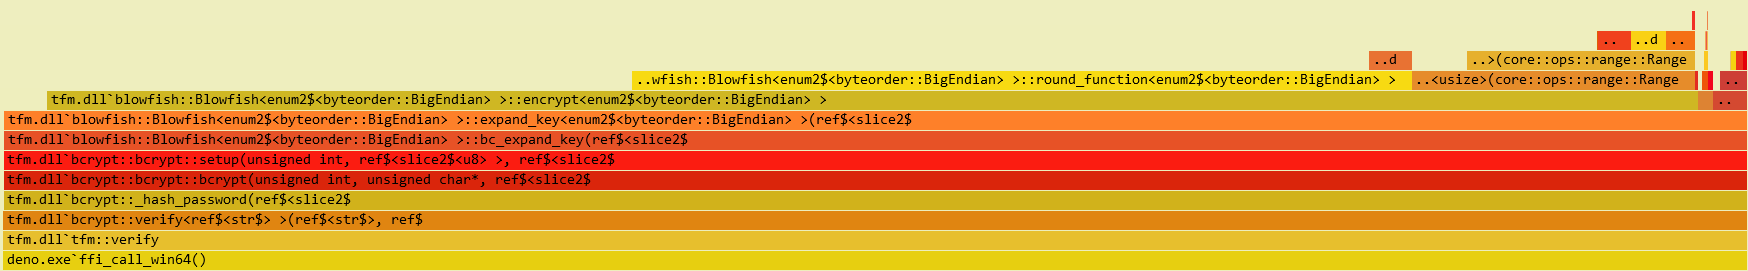
\includegraphics[width=\textwidth]{flamegraph}
    \caption{Flamegraph of the verify function.}
    \label{img:flamegraph}
\end{figure*}


\subsection{Where WASM fits}

WASM, as mentioned before, is quite useful in the browser, where it belongs. Right now, it is still in its early stages, and the WASM API within the browser is still young. The WASI libc library works, but it is not fully matured yet.

This is cobered in a Github issue. \cite{WASMBAD}

\begin{itemize}
    \item No way to control in a guaranteed fashion when new memory commit vs address space reserve occurs.
    \item No way to uncommit used memory pages.
    \item No way to shrink the allocated Wasm Memory.
    \item No virtual memory support (leading applications to either expect to always be able to grow, or have to implement memory defrag solutions)
    \item If Memory is Shared, then application needs to know the Maximum memory size ahead of time, or gratuitously reserve all that it can.
\end{itemize}

The author summarizes the issue by saying, \textit{you can only grab more memory, with no guarantee if the memory you got is a reserve or a commit}.

In WASM there is not way to allocate memory in compile time, witch would be benefitial for this project. WASM not being able to provide this functionality is a big limitation for this project, and results in a poorer performance.

\subsection{The data}

Let's take a look at the actual data to see if this idea actually holds up. These tests have been conducted using strings from a collection of 36 characters repeated 1,000 times to the same collection of 36 characters repeated 2,000 times. Each set is repeated 15 times, and the average is calculated to rule out any errors.

The data is collected sequentially, meaning that no async functions are used and the Deno and Rust functions are run one after the other to rule out any OS-induced noise.

\subsubsection{Hardware used}

These tests have been run on a broad range of hardware, all of the \verb|x86_64| architecture.

\begin{itemize}
    \item GitHub Actions builders 2-core CPU \verb|x86_64| \cite{Github}
    \item i9-12900H
    \item i5-1135G7
\end{itemize}

The data presented in this document will come from the CPU \textbf{i9-12900H}. However, there is data available in the GitHub repository that can be extracted from every commit added to the repo.

In every test run, the results are consistent but with obvious speed differences, as the selected hardware varies widely.

The \textbf{i9-12900H} is a 16-core CPU with 24 threads. It has a base clock of 2.2 GHz and a boost clock of 4.9 GHz. It has 24 MB of L3 cache and 16 MB of L2 cache. It is a very powerful CPU, and has a powerful single core performance. This means that it will go in favor of Deno. As reducing the speed of the processor will result in higher time values for Deno.

\subsubsection{Hashing}

The first part of the library to analyze is hashing. The algorithm used for hashing is bcrypt. This algorithm is a slow hashing algorithm that is designed to hash passwords. It is intentionally slow to prevent brute-force attacks \cite{Bcrypt}. The algorithm can be configured to use a different "cost," which is the number of iterations that the algorithm will perform. The higher the cost, the more secure the hash will be, but this comes at the expense of time. It also includes a salt to prevent rainbow table attacks.

\begin{figure}[H]
    \centering
    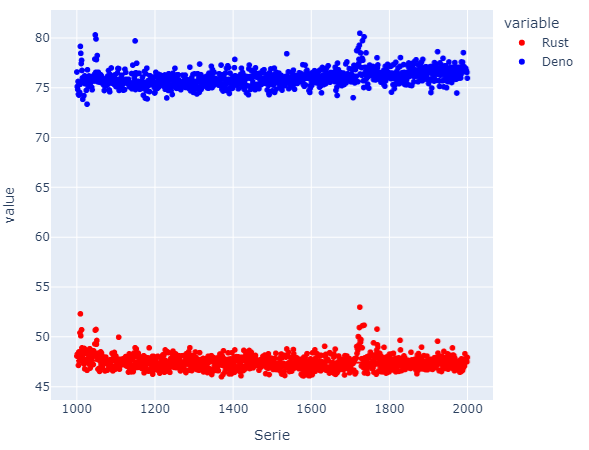
\includegraphics[width=0.52\textwidth]{hashing_lines}
\end{figure}

In this image, the creation of 1,000 hashes and their respective costs in milliseconds are shown, using a bcrypt cost of 14. On average, Rust is faster by \textbf{57\%}. Reducing the hardware choice to \textbf{i5-1135G7} results in a \textbf{34\%} more slowdown of Deno compared to Rust. Reducing even more the hardware to a single core instance of a VM runing on DigitalOcean, the results are even more drastic, with a \textbf{58\%} slowdown of Deno compared to Rust. This results are consistants with the rest of tests runned.

In this hash graph a small OS induced noise can be seen, and ruled out as Deno or Rust fault. At the start of the series and between 1600 and 1800 can be detected. As both timings go up it is safe to rule out this data pasing to the next section.
The trends here are not clearly defined, but two aspects are apparent from the following graphs.

\begin{figure}[H]
    \centering
    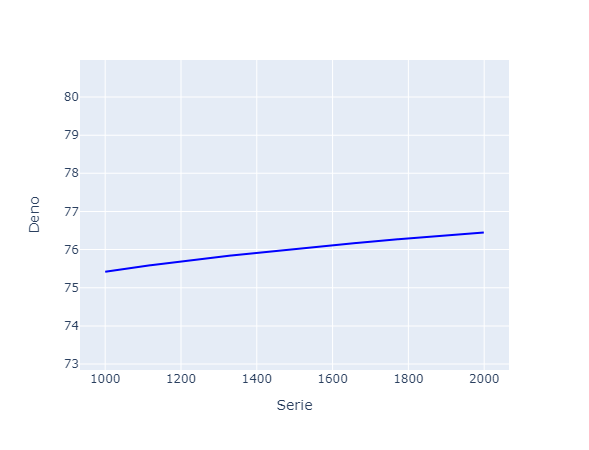
\includegraphics[width=0.52\textwidth]{trend_hash_deno}
\end{figure}

\begin{figure}[H]
    \centering
    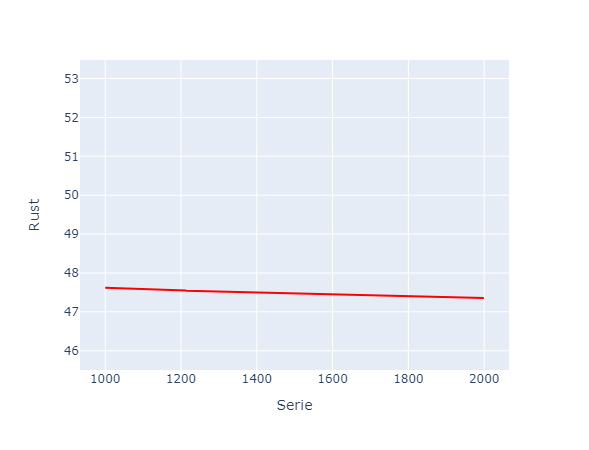
\includegraphics[width=0.52\textwidth]{images/trend_hash_rust.png}
\end{figure}

From the data, some observations can be made:
\begin{itemize}
    \item The cost of hashing will increase more rapidly than it does in Rust.
    \item Rust will be more stable and experience less growth.
\end{itemize}

The growth rate in the Deno is \textbf{0.001} and in Rust is in the range of the data chosen negible. Pushing it all the way to \textbf{1.800.000} characters will result in a growth rate of \textbf{0.0001}.

\subsubsection{Secret boxes}

Secret boxes are a concept introduced by the library NaCl. A secret box is essentially a box with only one lock, serving as a metaphor for synchronous cryptography. The algorithm to be used in this project is a variant called \textit{tweetnacl}, which replicates the exact functionality of NaCl but fits within 100 tweets.

The focus of this library is on speed and minimal disk footprint for both developers and users.

\begin{figure}[H]
    \centering
    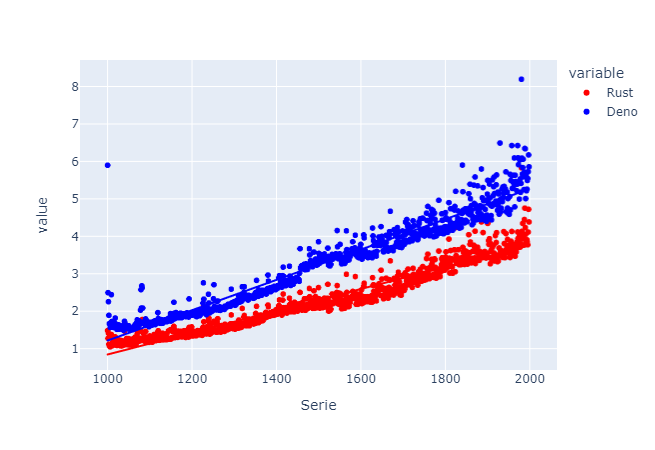
\includegraphics[width=0.52\textwidth]{images/secretbox_lines}
\end{figure}

In the graph, there are some Deno results that deviate from the predicted outcomes. Since these anomalies do not appear in the Rust variant, they likely arise from variations in V8's \textit{heat} function. In V8, when a function is called, it gains \textit{heat}, meaning it gets cached for later use. If a function is executed frequently, it gets stored in machine code to maximize performance.

In this example, it can once again be observed that JavaScript is more unstable than Rust and tends to experience greater growth in computational cost.

\begin{figure}[H]
    \centering
    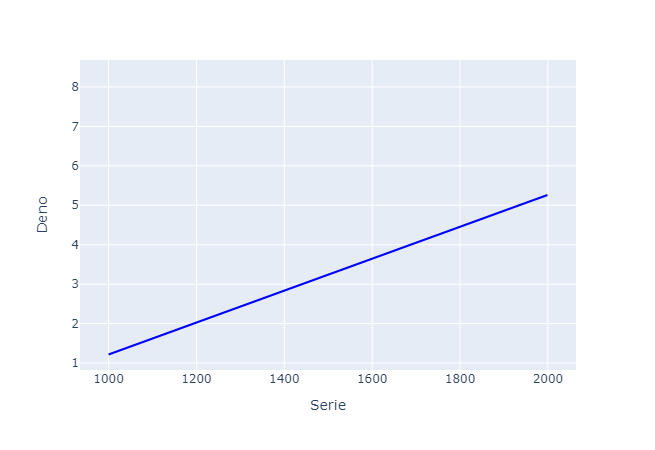
\includegraphics[width=0.52\textwidth]{trend_secretbox_deno}
\end{figure}

\begin{figure}[H]
    \centering
    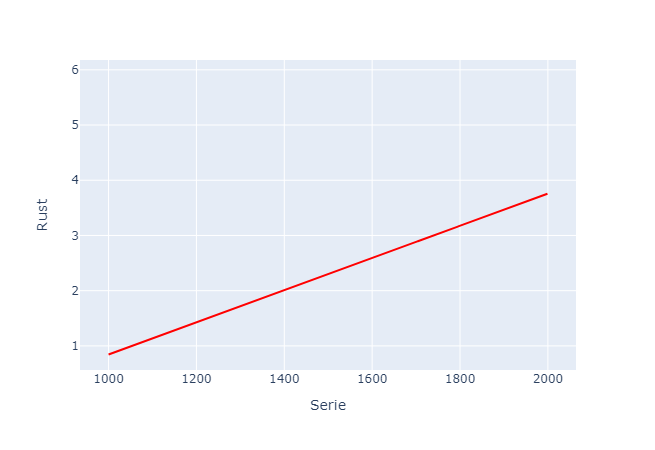
\includegraphics[width=0.52\textwidth]{images/trend_secretbox_rust}
\end{figure}

From the data, some observations can be made:
\begin{itemize}
    \item The cost of encrypting will rise more rapidly in JavaScript than it does in Rust.
    \item Rust will be more stable and experience less growth.
\end{itemize}

The growth rate in the Deno is \textbf{0.004} and in Rust is \textbf{0.003}.

\subsubsection{Box}

A box is essentially a container with two locks, serving as another metaphor for asymmetric encryption. Like the previous algorithm, this one is based on \textit{tweetnacl}.

\begin{figure}[H]
    \centering
    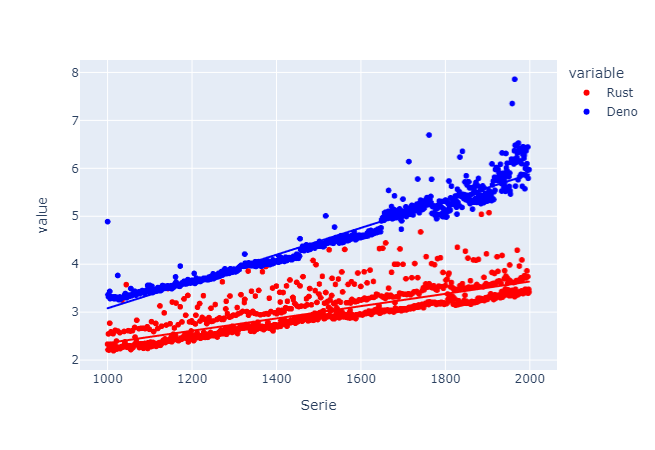
\includegraphics[width=0.52\textwidth]{images/box_lines}
\end{figure}

In this final algorithm, Rust outperforms Deno significantly, even though its performance is more dispersed.

\begin{figure}[H]
    \centering
    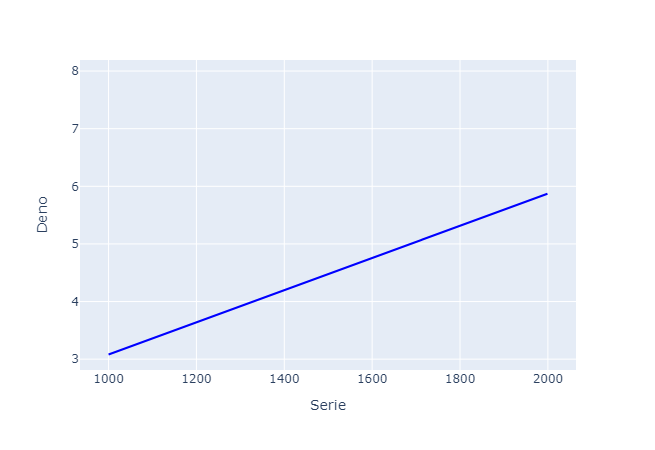
\includegraphics[width=0.52\textwidth]{trend_box_deno}
\end{figure}

\begin{figure}[H]
    \centering
    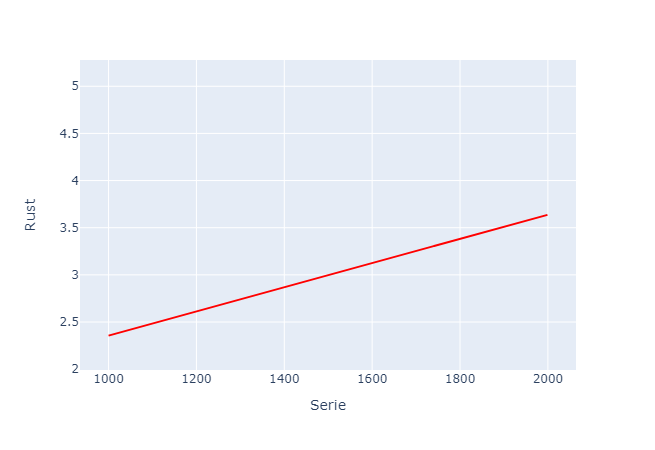
\includegraphics[width=0.52\textwidth]{images/trend_box_rust}
\end{figure}

From the data, some aspects can be deduced:
\begin{itemize}
    \item The cost of encrypting will rise more rapidly in Deno than in Rust.
    \item Rust will be more stable and experience less growth.
\end{itemize}

The growth rate in the Deno is \textbf{0.003} and in Rust is \textbf{0.001}.

\section{Conclusions}

The objective of this project has been met with remarkable success, both theoretically and pragmatically. The initiative was principally driven by the need to enhance the efficiency of JavaScript-based projects, a technology that is increasingly becoming ubiquitous. One notable application of this effort is seen in the InterPlanetary File System (IPFS) \cite{IPFS}, which heavily relies on our optimized suite of algorithms for its operations. Particularly, this suite of libraries plays a pivotal role in the functionality of OrbitDB, an instrumental library employed for the creation of decentralized databases.

\subsection{Technical Overview}

The libraries developed under this project are predicated on distributed technology paradigms. These paradigms operate on the principle of data transmission involving multiple peers, wherein each peer sends fractional pieces of information to a centralized entity. Given this architecture, the need for high-speed data aggregation and dissemination is critical. Such requirements present unique challenges when relying on traditional methods of information transport.

\subsection{Performance Limitations in IPFS}

Although IPFS is fundamentally a JavaScript-based project, it is not immune to the performance bottlenecks commonly associated with the language. Despite commendable optimization efforts by the IPFS development team, the potential of the system is constricted by the inherent limitations of JavaScript.

A considerable breakthrough was achieved when IPFS was implemented in the Go programming language, known for its C Application Binary Interface (ABI) and robust WebAssembly (WASM) capabilities. Nevertheless, the core functionalities still rely on JavaScript. While multiple implementations of the IPFS protocol exist, the official version remains the most extensively deployed, resulting in significant network latency.

\subsection{Performance Augmentation}

The integration of our library promises to drastically improve performance metrics, both in desktop applications and browser-based environments.

\subsection{Future-Proofing Developer Environments}

In this project, it is made enphasis in the use of Deno because of its sandboxed environment. The next logical step to prevent malicious code from being executed in developers machines is the use of containers. This way, the developer can be sure that the code is not doing anything malicious. Through the utilization of Docker containers. This virtualization allows for a consistent and reproducible development atmosphere, replete with all the necessary dependencies. It also serves as a security measure, as the operational codebase resides within a contained environment, effectively neutralizing potential threats.

\subsection{Industry Leadership}

Microsoft is at the forefront of this technological space, particularly with their innovative feature in Visual Studio Code known as Remote Containers. This utility allows developers to execute code within a containerized environment directly from a specific folder, obviating the need for local dependency installations. This feature is not just advantageous for enhancing the developer experience but also critically important for bolstering security protocols.

Microsoft offers a local version of this feature, named \verb|dev-containers|, that provides identical functionalities but operates within a locally-hosted environment.

\bibliographystyle{unsrt} % We choose the "plain" reference style
\bibliography{refs} % Entries are in the refs.bib file
\end{document}